\begin{figure}[H]
\centering
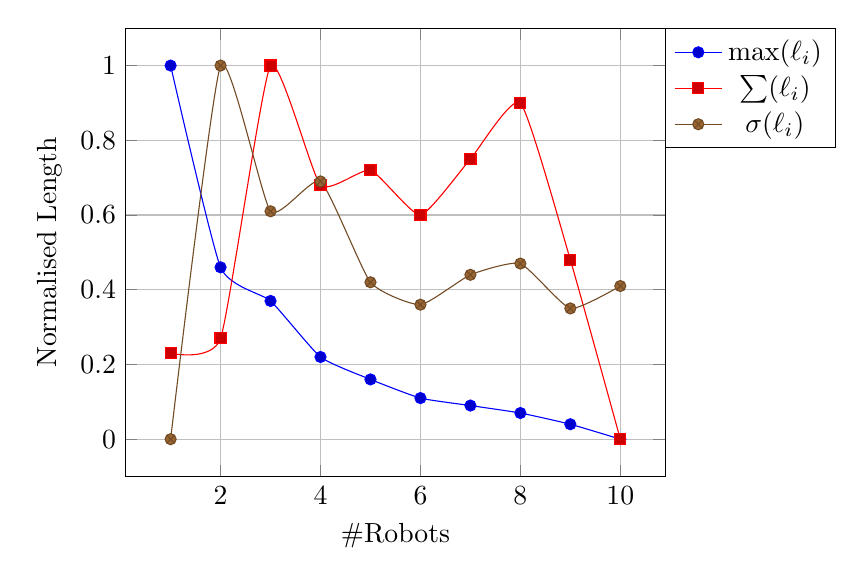
\begin{tikzpicture}
	\begin{axis}[
%		height=9cm,
%		width=9cm,
		grid=major,
                legend style = {at={(1,1)}, anchor=north west},
		xlabel=\#Robots,
		ylabel=Normalised Length,
		smooth,
		tension=0.3
	]

	\addplot coordinates {
(1, 1.00)
(2, 0.46)
(3, 0.37)
(4, 0.22)
(5, 0.16)
(6, 0.11)
(7, 0.09)
(8, 0.07)
(9, 0.04)
(10, 0.00)
	};
	\addlegendentry{$\max(\ell_i)$}

	\addplot coordinates {
(1, 0.23)
(2, 0.27)
(3, 1.00)
(4, 0.68)
(5, 0.72)
(6, 0.60)
(7, 0.75)
(8, 0.90)
(9, 0.48)
(10, 0.00)
	};
	\addlegendentry{$\sum(\ell_i)$}

	\addplot coordinates {
(1, 0.00)
(2, 1.00)
(3, 0.61)
(4, 0.69)
(5, 0.42)
(6, 0.36)
(7, 0.44)
(8, 0.47)
(9, 0.35)
(10, 0.41)

	};
	\addlegendentry{$\sigma(\ell_i)$}
	\end{axis}
\end{tikzpicture}
\caption[Perform. indexes increasing the \#robots, 15x15 grid using NC]{Performance indexes increasing the num. of robots, 15x15 grid using NC}
\end{figure}